\documentclass[12pt,a4paper]{article} 

\usepackage[spanish]{babel} 
\usepackage[utf8]{inputenc}
\usepackage[numbers,sort&compress]{natbib}
\usepackage{graphicx} 
\usepackage{graphics} 
\usepackage{amsfonts}
\usepackage[left=2cm,right=2cm,top=2cm,bottom=2cm]{geometry}
\usepackage{listings}
\usepackage[usenames,dvipsnames]{color}
\usepackage{subfig}
\usepackage{natbib}
\author{Paola Lizbeth Vázquez}

\title{Matemáticas Computacionales \\ Práctica 2: Estudio de una base de datos} 
\author{Profesor: Ángel Isabel Moreno Saucedo \\ Alumno: Paola Lizbeth Vázquez Leal \\ Semestre Febrero - Junio 2021}
\date{}

\begin{document}
\maketitle
Práctica 2
\section{Introducción}

 En esta actividad se analizará una Base de datos elegida por el estudiante. De esta se observarán los atributos de cada uno así como tambien se mostrara graficamente dichas observaciones. Además se analizarán los datos de una sola variable y de dos variables de igual manera. La base de datos elegida es llamada trees, que contiene informacion de medidas de un tipo de árbol conocido como Prunus serotina  \citep{plants}.


\section{Base de datos: identificación de árboles de cerezo negro.}

  La base de datos \textbf{trees} contiene 31 observaciones del tipo  árbol de cerezo, siendo este el árbol de cerezo negro como nos proporciona \citep{PTR}. Nos proporciona las mediciones del diametro, la altura y el volumen de la madera de 31 árboles. Dentro de la base de datos nos proporcionan Girth, sin embargo está mal representado ya que este en realidad es una medida hecha de 4 a 6 pies sobre el suelo. 

Los atributos de esta base de datos son 3:

\begin{enumerate}
\item Girth
\item Height
\item Volume
\end{enumerate}



\subsection{Estadística de una variable}
Para comenzar con la descripción de una variable, contamos con tres tipos de atribustos, los cuales han sido mencionados antes. Los datos obtenidos de Girth  (diametro) son un mínimo de 8.30 y un máximo de 20.60, en cuanto a su media de  12.90 y mediana de 13.25. Los datos de Height (altura) con un mínimo de 63 y un máximo de 87, en cuanto a su media y mediana son iguales con 76. Por ultimo los datos de Volume (volumen) son un mínimo de 10.20 y un máximo de 77.00. Para ello se encuentran las gráficas de densidad que nos mostraran los datos antes platicados.
Además podemos agregar la grafica de caja de bigotes [\ref{fig:cajab}], donde podemos apreciar con mayor claritud donde se encuentra la media dada por la diferencia del ranfo intercuartil.


\begin{figure}
\centering
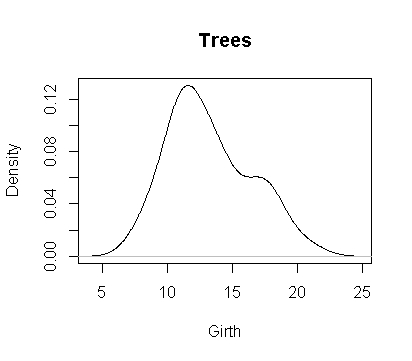
\includegraphics[scale=0.9]{Densidad1}
\caption{ Densidad respecto al atributo Diametro.}
\end{figure}

\begin{figure}
\centering
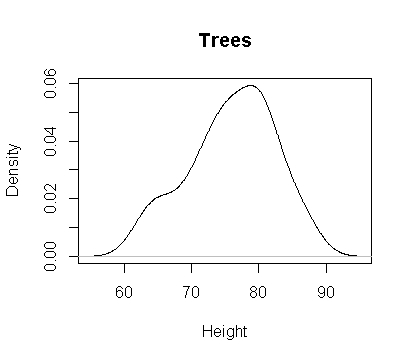
\includegraphics[scale=0.9]{Densidad2}
\caption{ Densidad respecto al atributo Altura.}
\end{figure}

\begin{figure}
\centering
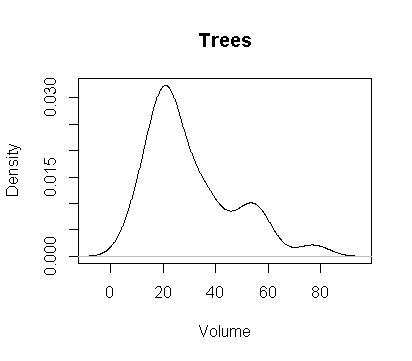
\includegraphics[scale=0.9]{Densidad3}
\caption{ Densidad respecto al atributo Volumen.}
\end{figure}

\begin{figure}
\centering
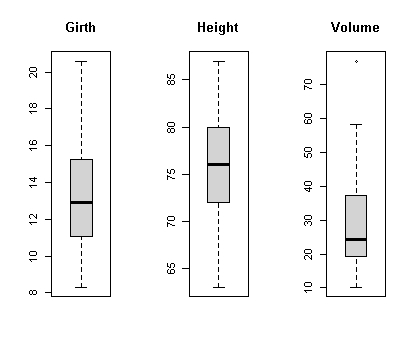
\includegraphics[scale=0.9]{cajab}
\caption{ Muestra de la media junto al primer y tercer intercuartil.  }
\label{fig:cajab}
\end{figure}
 
\newpage
\subsection{Estadística de dos variables}
De la figura [\ref{fig:cor}] podemos notar como las variables de Girth y Volume se encuentran fuertemente correlacionadas la una con la otra, esto significa que si una de las variables dismunuye su tamaño la otra tambien lo hará, así como tambien pueden aumentar. En este caso donde la variable (llamémoslas 1 a Girth y 2 a Volume respectivamente)1 por lo que, si una de las variables disinuye, lo hará la otra. Mientras que la altura (height) esta altamente correlacionada con el volumen como se muestra en la figura [\ref{fig:disp3}] mientras que con el diametro (Girth) está medianamente relacionada como se ve en la figura [\ref{fig:disp2}].   
\citep{repositorio}


\begin{figure}
\centering
\includegraphics[scale=0.9]{cor}
\caption{}
\label{fig:cor}
\end{figure}

\begin{figure}
\centering
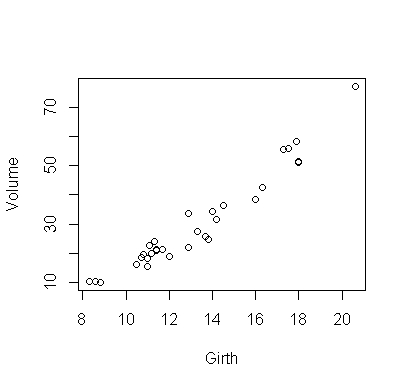
\includegraphics[scale=0.9]{disp1}
\caption{Dispersión existente entre diametro y altura}
\label{fig:disp1}
\end{figure}

\begin{figure}
\centering
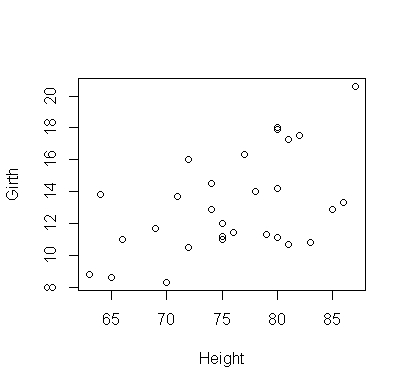
\includegraphics[scale=0.9]{disp2}
\caption{Dispersión existente entre  altura y diametro}
\label{fig:disp2}
\end{figure}

\begin{figure}
\centering
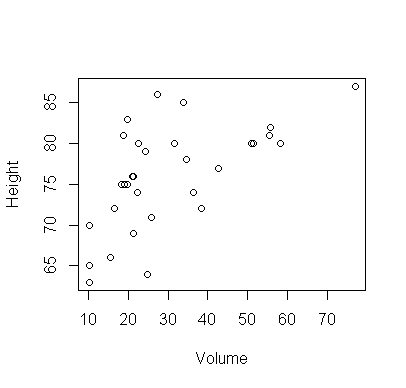
\includegraphics[scale=0.9]{disp3}
\caption{Dispersión existente entre volumen y altura}
\label{fig:disp3}
\end{figure}

\newpage
\section{Conclusión}
La base de datos de trees o bien conocida como trees black cherry, se usa como referencia a las mediciones de dichos árboles, llevando un listado de cada árbol que fue medido y relacionado a este tipo. Como se pudo observar los datos que esta base contenia fueron de ayuda al momento de buscar la información que era pedida para realizar la actividad. En ella se pudo observar que los tres atributos estaban correlacionados entre sí, aunque unos más que otros como fue el caso de Girth y Valume, mediante las graficas esta información pudo ser comprobada al igual que con los demás casos. En cuanto al momento de realizar el codigo, como se podra observar en él, la relación de porcentaje con la frecuencia decidí obtener esta individualmente, ya que la base no tenía ningún clase factor. \citep{handbook}

\newpage
\bibliography{bibliografia}
\bibliographystyle{plainnat}


\end{document}